% Copyright (C) 2017 - Michael Baudin

  \documentclass{beamer}

%\setbeameroption{hide notes}
%\setbeameroption{show notes}
%\setbeameroption{show only notes}

  % Copyright (C) 2012 - EDF R&D - Michael Baudin

% To highlight source code
\usepackage{listings}
\definecolor{darkgreen}{rgb}{0,0.5,0}
\definecolor{violet}{rgb}{0.5,0,1}

\usepackage{lmodern}% http://ctan.org/pkg/lm

\usetheme{Montpellier}
\setbeamertemplate{navigation symbols}{} % Remove navigation
\useoutertheme{infolines}

\usepackage[utf8]{inputenc}
\usepackage[T1]{fontenc}

%\usepackage[french]{babel}
%\uselanguage{French}
%\languagepath{French}

\def\bx{{\bf x}}
\def\RR{\mathbb{R}}

\newcommand{\pyvar}[1]{\texttt{#1}}

\def \ot {OpenTURNS}

\hypersetup{colorlinks=true}

\usepackage{adjustbox}

\title[OpenTURNS]{The OpenTURNS uncertainty quantification library}

\author[Baudin et al.]{
Michaël Baudin \inst{1} \and
Julien Schueller \inst{2}
}

\institute[EDF-Phiméca]{
\inst{1} EDF R\&D. 6, quai Watier, 78401, Chatou Cedex - France, michael.baudin@edf.fr \and %
\inst{2} Phimeca Engineering. 18/20 boulevard de Reuilly, 75012 Paris - France, schueller@phimeca.com
}

\date[]{EuroSciPy 2017, Erlangen, Germany}

%%%%%%%%%%%%%%%%%%%%%%%%%%%%%%%%%%%%%%%%%%%%%%%%%%%%%%%%%%%%%%%%%%%%%%%%%%%%%

  \begin{document}

%%%%%%%%%%%%%%%%%%%%%%%%%%%%%%%%%%%%%%%%%%%%%%%%%%%%%%%%%%%%%%%%%%%%%%%%%%%%%

  \begin{frame}
  \titlepage
  
  \begin{columns}
    \column{0.45\textwidth}
  \begin{center}

\includegraphics[height=0.15\textheight]{figures/logo-edf.jpg}
\end{center}
    \column{0.1\textwidth}
	
    \column{0.45\textwidth}
  \begin{center}

\includegraphics[height=0.15\textheight]{figures/logo-phimeca.png}
\end{center}
  \end{columns}

  \end{frame}

%%%%%%%%%%%%%%%%%%%%%%%%%%%%%%%%%%%%%%%%%%%%%%%%%%%%%%%%%%%%%%%%%%%%%%%%%%%%%

\begin{frame}
\frametitle{Contents}
\tableofcontents
\end{frame}

%%%%%%%%%%%%%%%%%%%%%%%%%%%%%%%%%%%%%%%%%%%%%%%%%%%%%%%%%%%%%%%%%%%%%%%%%%%%%
\section{Uncertainty Quantification Methodology}

%%%%%%%%%%%%%%%%%%%%%%%%%%%%%%%%%%%%%%%%%%%%%%%%%%%%%%%%%%%%%%%%%%%%%%%%%%%%%

\begin{frame}
\frametitle{Uncertainty Quantification Methodology}

\begin{center}
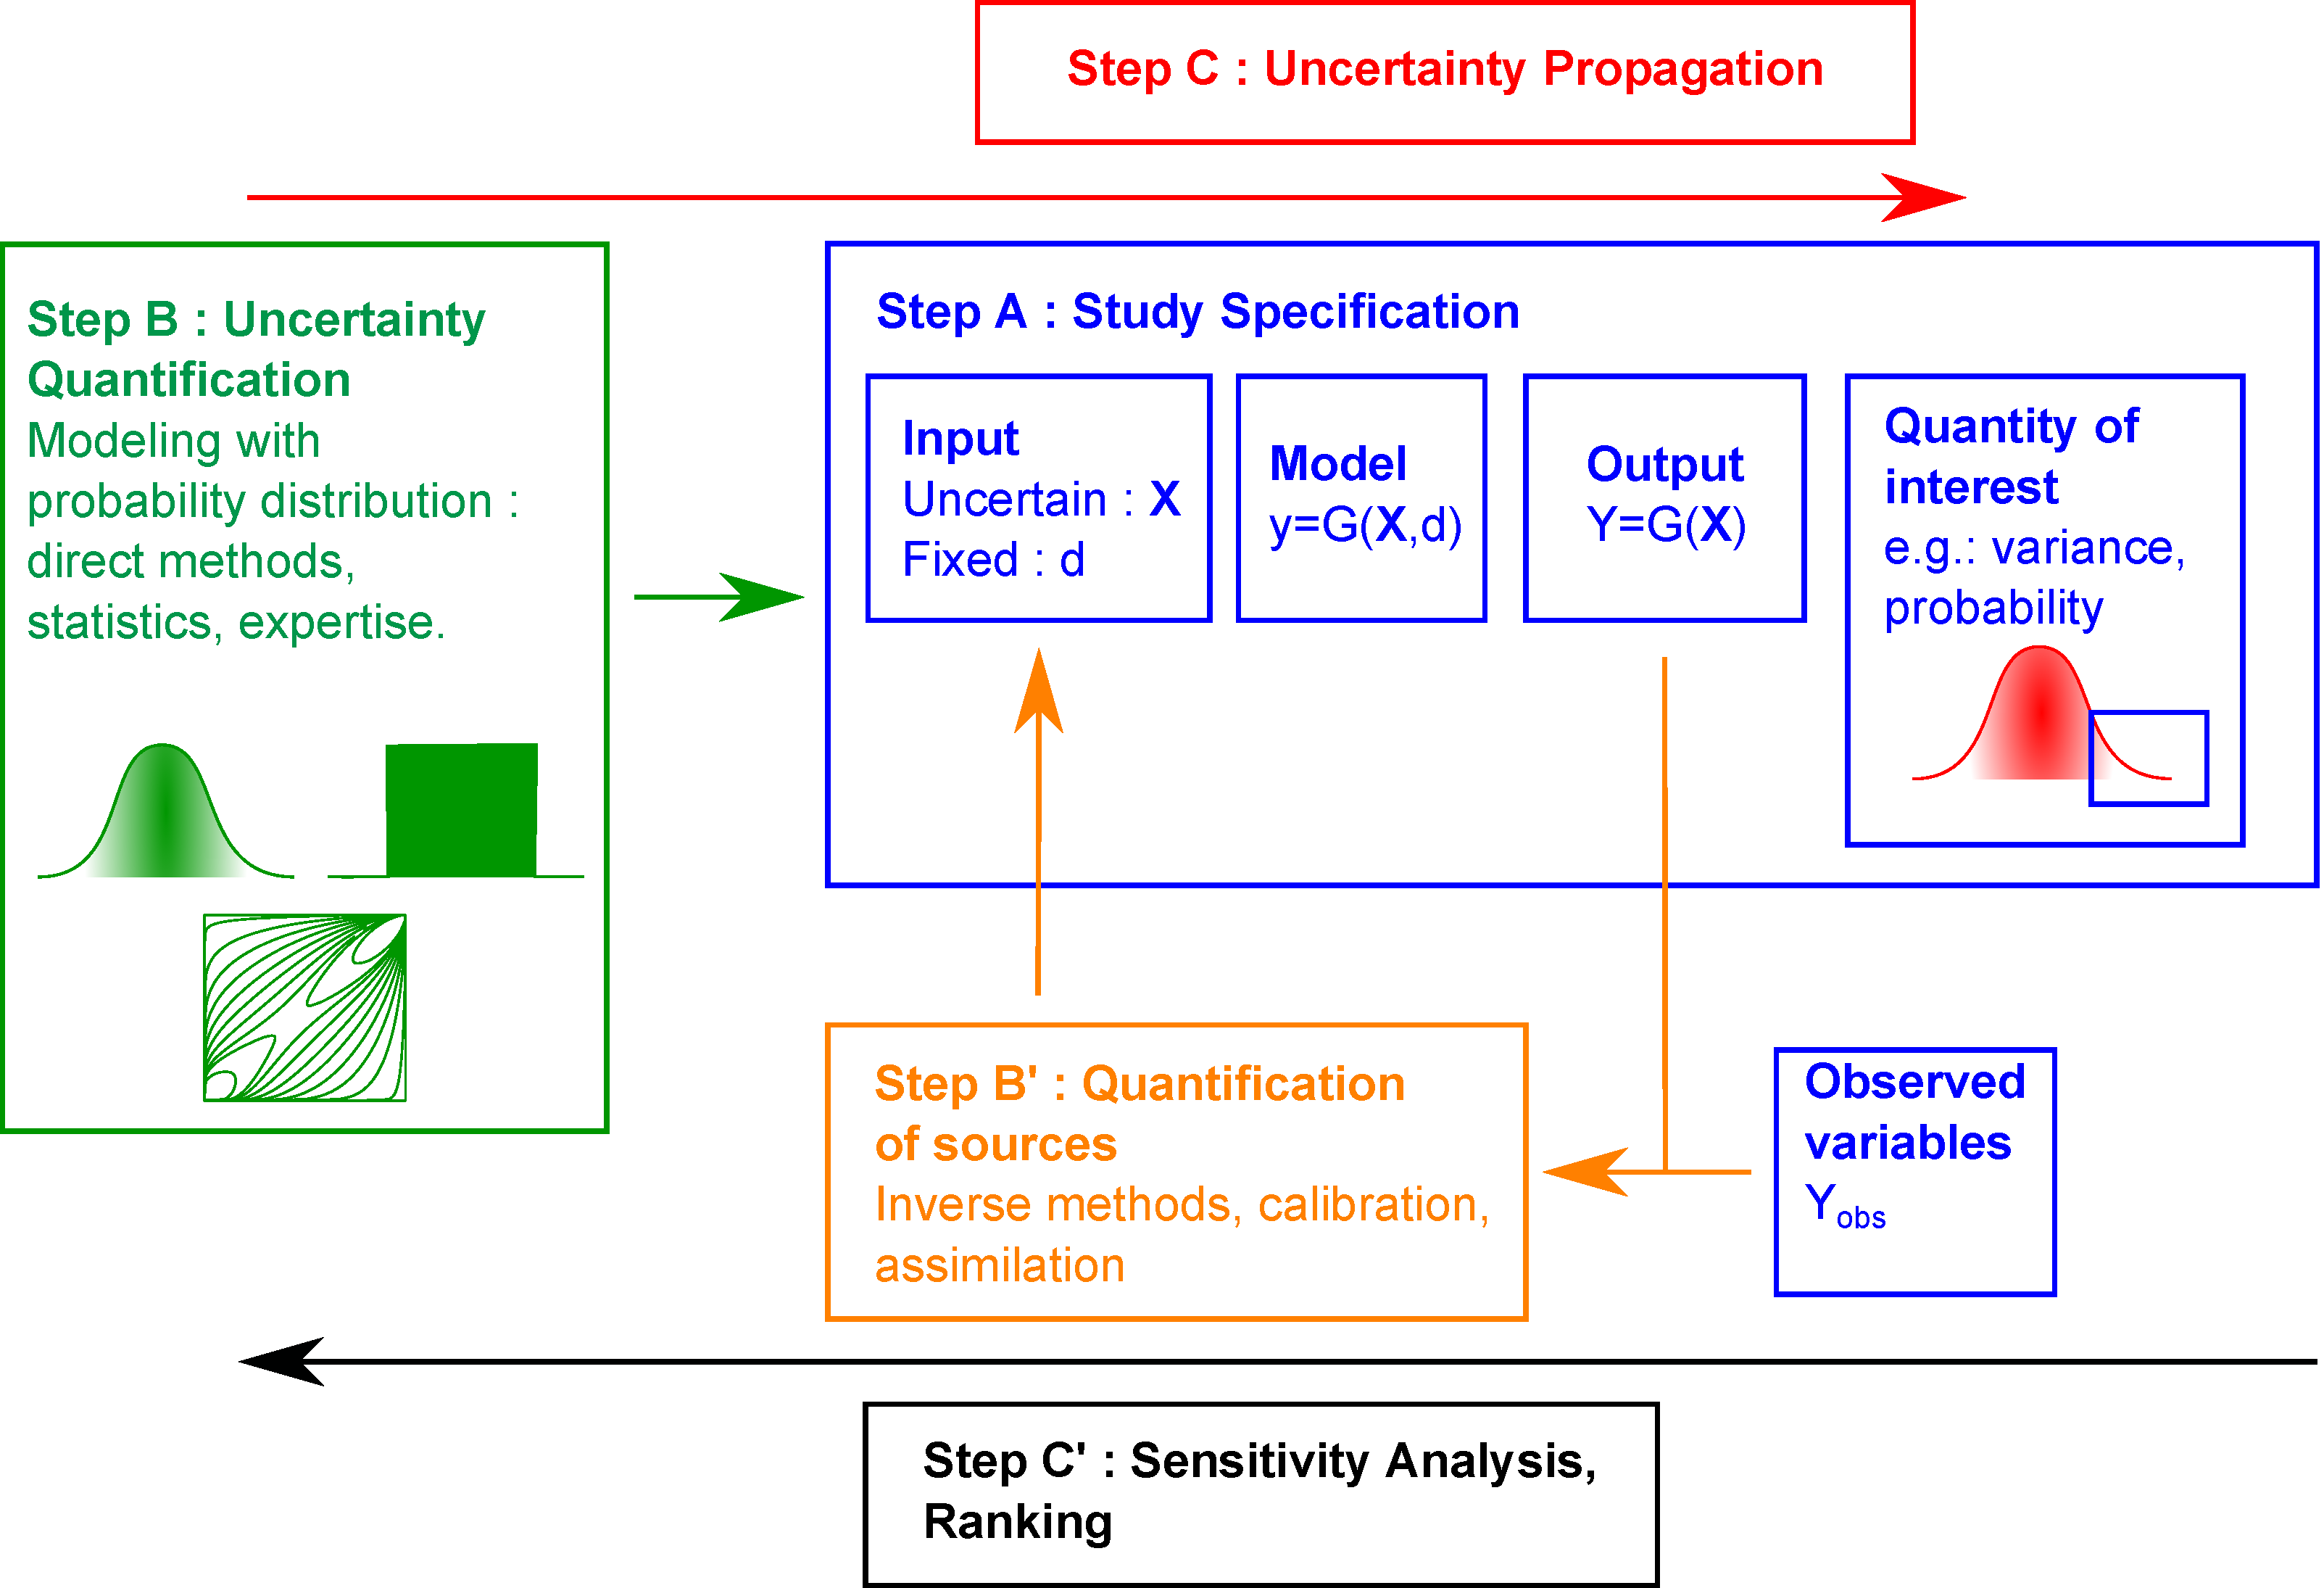
\includegraphics[width=0.9\textwidth]{figures/MethodologieIncertitude-EN}
\end{center}

\end{frame}


%%%%%%%%%%%%%%%%%%%%%%%%%%%%%%%%%%%%%%%%%%%%%%%%%%%%%%%%%%%%%%%%%%%%%%%%%%%%%
\section{The OpenTURNS library}

%%%%%%%%%%%%%%%%%%%%%%%%%%%%%%%%%%%%%%%%%%%%%%%%%%%%%%%%%%%%%%%%%%%%%%%%%%%%%

\begin{frame}
\frametitle{\ot{}}

  \begin{columns}
    \column{0.6\textwidth}
	
\begin{itemize}
\item Uncertainty quantification, uncertainty propagation, sensitivity analysis and metamodeling
\item Partners : EDF, Phiméca, Airbus, IMACS
\item \url{www.openturns.org}
\item Licence LGPL 
\item Linux, Windows
\end{itemize}

    \column{0.4\textwidth}

	\begin{center}
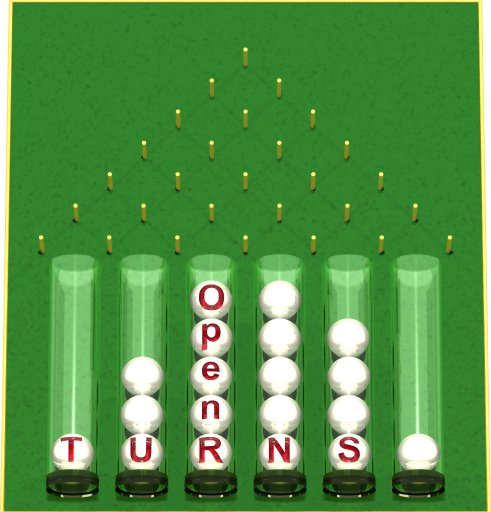
\includegraphics[width=0.9\textwidth]{figures/logo-ot}
\end{center}

	\end{columns}
\end{frame}

%%%%%%%%%%%%%%%%%%%%%%%%%%%%%%%%%%%%%%%%%%%%%%%%%%%%%%%%%%%%%%%%%%%%%%%%%%%%%

\begin{frame}[containsverbatim]

Overview :
  \begin{columns}
    \column{0.5\textwidth}
\frametitle{\ot{}}
\begin{itemize}
\item First release: 2007
\item technical committee (including 4 developers), steering committee
\item Users: mainly in France
\item Number of users: $\approx 1000$ (10900 Conda downloads in 2016-2017)
\end{itemize}

    \column{0.5\textwidth}

\frametitle{\ot{}}
\begin{itemize}
\item Size of the project (2017): 5420 files, 680 classes, 158k sloc
\item Documentation: theoric, API, developer
\end{itemize}

\end{columns}

\end{frame}

%%%%%%%%%%%%%%%%%%%%%%%%%%%%%%%%%%%%%%%%%%%%%%%%%%%%%%%%%%%%%%%%%%%%%%%%%%%%%

\begin{frame}[containsverbatim]
\frametitle{Features overview 1/2}

  \begin{columns}
    \column{0.5\textwidth}
Data analysis:
\begin{itemize}
\item Visual analysis
\item (Non)parametric estimation
\item Distribution fitting tests
\item Bayesian calibration
\end{itemize}

    \column{0.5\textwidth}

Probabilistic modeling:
\begin{itemize}
\item Dependence modeling: Copulas
\item Univariate \& multivariate distributions
\item Process: ARMA, Gaussian
\end{itemize}

\end{columns}

\end{frame}


%%%%%%%%%%%%%%%%%%%%%%%%%%%%%%%%%%%%%%%%%%%%%%%%%%%%%%%%%%%%%%%%%%%%%%%%%%%%%

\begin{frame}[containsverbatim]
\frametitle{Features overview 2/2}

  \begin{columns}
    \column{0.5\textwidth}
Meta modeling:
\begin{itemize}
\item Visual analysis
\item Gaussian process regression (Kriging)
\item Spectral methods: Functional chaos expansion, Karhunen-Loeve, low-rank tensors
\item Bayesian calibration
\end{itemize}

    \column{0.5\textwidth}

Reliability, sensitivity:
\begin{itemize}
\item Monte Carlo, LHS, low-discrepancy sequences
\item Variance reduction methods: importance sampling, subset sampling
\item Approximation methods: FORM, SORM
\item Indices: Spearman, Sobol, ANCOVA
\end{itemize}

\end{columns}

\end{frame}


%%%%%%%%%%%%%%%%%%%%%%%%%%%%%%%%%%%%%%%%%%%%%%%%%%%%%%%%%%%%%%%%%%%%%%%%%%%%%

\section{Example}

\begin{frame}[containsverbatim]
\frametitle{Flood example 1/5}

The flood model of a river compares the water level to the dike height:

$$S = \left(\frac{Q}{Ks\times300\times\sqrt{(Zm-Zv)/5000}}\right)^{3/5}+Zv-55.5-3$$


\begin{center}
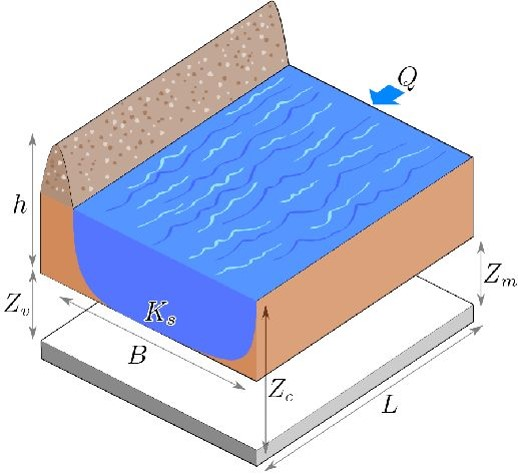
\includegraphics[width=0.5\textwidth]{figures/crue}
\end{center}

\end{frame}

%%%%%%%%%%%%%%%%%%%%%%%%%%%%%%%%%%%%%%%%%%%

\begin{frame}[containsverbatim]
\frametitle{Flood example 2/5}

\begin{itemize}
\item Q $\sim$ Gumbel(alpha=0.00179, beta=1013), flow rate [$m^3s^{-1}$]
\item Ks $\sim$ Normal(mu=30.0, sigma=7.5), strickler [$m^{1/3}s^{-1}$]
\item Zv $\sim$ Uniform(a=49, b=51), downstream depth [m]
\item Zm $\sim$ Uniform(a=54, b=56), upstream depth [m]
\end{itemize}

Failure occurs when S is positive, lets estimate $P_f ={\mathbb P}\left( S(\underline{X}) > 0 \right)$.

\end{frame}

\begin{frame}[containsverbatim]
\frametitle{Flood example 3/5}

\lstset{language=python}

\begin{lstlisting}
# Probabilistic model
Q = ot.Gumbel(1./558., 1013.)
Ks = ot.Normal(30.0, 7.5)
Zv = ot.Uniform(49.0, 51.0)
Zm = ot.Uniform(54.0, 56.0)
copula = ot.IndependentCopula(4)
dist = ot.ComposedDistribution([Q, Ks, Zv, Zm], copula)
\end{lstlisting}

\begin{center}
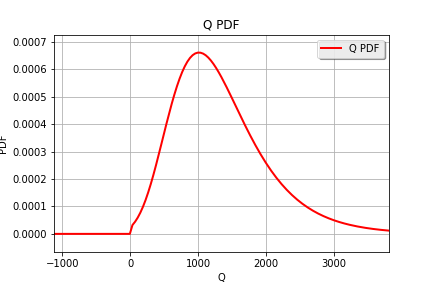
\includegraphics[width=0.5\textwidth]{figures/q_dist}
\end{center}

\end{frame}






\begin{frame}[containsverbatim]
\frametitle{Flood example 4/5}

\lstset{language=python}
\begin{lstlisting}
# Random variable S=G(Q,Ks,Zv,Zm)
rv = ot.RandomVector(dist)
f = ot.SymbolicFunction(['Q', 'Ks', 'Zv', 'Zm'],
  ['(Q/(Ks*300.*sqrt((Zm-Zv)/5000)))^(3.0/5.0)+Zv-55.5-3.'])
S = ot.CompositeRandomVector(f, rv)
\end{lstlisting}

\begin{center}
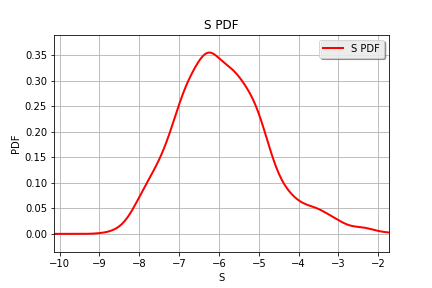
\includegraphics[width=0.5\textwidth]{figures/s_dist}
\end{center}

\end{frame}








\begin{frame}[containsverbatim]
\frametitle{Flood example 5/5}

\lstset{language=python}
\begin{lstlisting}
# Compute P(S>0) using First Order Reliability Method algorithm
event = ot.Event(S, ot.Greater(), 0.0) # event S>0
optimAlgo = ot.Cobyla()
algo = ot.FORM(optimAlgo, event, dist.getMean())
algo.run()
result = algo.getResult()
print('Pf=', result.getEventProbability()) # P(S>0)=0.00053
result.drawImportanceFactors()
\end{lstlisting}

\begin{center}
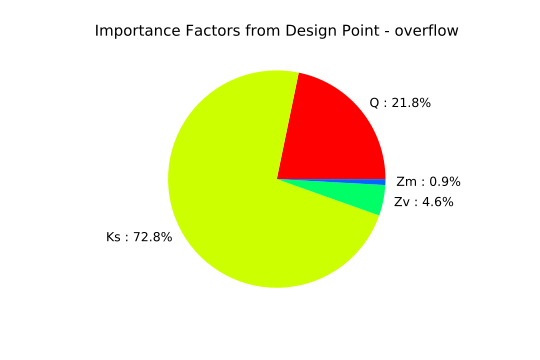
\includegraphics[width=0.6\textwidth]{figures/imp_fact}
\end{center}

\end{frame}

%%%%%%%%%%%%%%%%%%%%%%%%%%%%%%%%%%%%%%%%%%%%%%%%%%%%%%%%%%%%%%%%%%%%%%%%%%%%%

\section{Software architecture}

\begin{frame}[containsverbatim]
\frametitle{Architecture}

\begin{itemize}
\item C++ core / SWIG Python bindings
\item BLAS / LibXml2 / TBB / muParser / NLopt
\item Packaging: Debian, Conda, Windows
\item Compilation: cmake
\item Documentation: Sphinx
\item Repository: https://github.com/openturns
\end{itemize}

\end{frame}


%%%%%%%%%%%%%%%%%%%%%%%%%%%%%%%%%%%%%%%%%%%%%%%%%%%%%%%%%%%%%%%%%%%%%%%%%%%%%

\section{Modules}

\begin{frame}[containsverbatim]
\frametitle{Modules}

\begin{itemize}
\item C++/SWIG / pure Python

\item otrobopt: Robust optimization module

\item otfmi: FMI models manipulation

\item otsvm: SVM classifiers, metamodels

\item otagrum: Bayesian networks module

\item otwrapy: wrap external simulation codes

\item ...
\end{itemize}

Contributions welcome!

\end{frame}

%%%%%%%%%%%%%%%%%%%%%%%%%%%%%%%%%%%%%%%%%%%%%%%%%%%%%%%%%%%%%%%%%%%%%%%%%%%%%

\begin{frame}
\frametitle{END}

Thank you for your attention!

Any questions?

\begin{center}

\includegraphics[width=0.2\textwidth]{figures/logo-ot-small}
\end{center}

\end{frame}

% %%%%%%%%%%%%%%%%%%%%%%%%%%%%%%%%%%%%%%%%%%%%%%%%%%%%%%%%%%%%%%%%%%%%%%%%%%%%%

\section{Bibliography}

\begin{frame}
\frametitle{Bibliography}

\begin{itemize}
\item Airbus, EDF, Phimeca Engineering, IMACS. 
OpenTURNS, a scientific library usable as a Python module dedicated to the treatment of uncertainties, 
\url{www.openturns.org}.
\item Airbus, EDF, Phimeca Engineering, IMACS. Documentation of OpenTURNS, version 1.9. 
\url{http://openturns.github.io/openturns/1.9/contents.html}
\item  Michaël Baudin, Anne Dutfoy, Bertrand Iooss, and Anne-Laure Popelin. 
OpenTURNS: An Industrial Software for Uncertainty Quantification in Simulation, 
Handbook of Uncertainty Quantification, 
pages 1-38. Springer International Publishing, 2016
\item Open TELEMAC-MASCARET. 
Electricité de france, Sogreah, Hydraulic Research Wallingford, 
Centre d'Etudes Techniques Maritimes et Fluviales, Bundesanstalt fur Wasserbau, and Daresbury Laboratory.
\url{www.opentelemac.org}.
\end{itemize}

\end{frame}

\end{document}
